To test the pipeline, the user is able to select their own interferometer to test with, as well as a sky model that has knows positions and brightness.
% functionality was implemented 
% that allows the user to select their own interferometer array layout and sky model.
The user can then generate an image that that interferometer would see if it were to observe that sky model. If the image comes out similar to the sky model then the user knows the pipeline is working as intended. An example is given below: \\
Say the user were to select KAT-7\cite{KAT-7}, which is a real interferometer that we have created a model of to use in our experiments, as the interferometer and select the sky model in figure \ref{fig:line_model}.

\begin{figure}[H]
  \centering
  \begin{subfigure}[b]{0.49\textwidth}
    \centering
    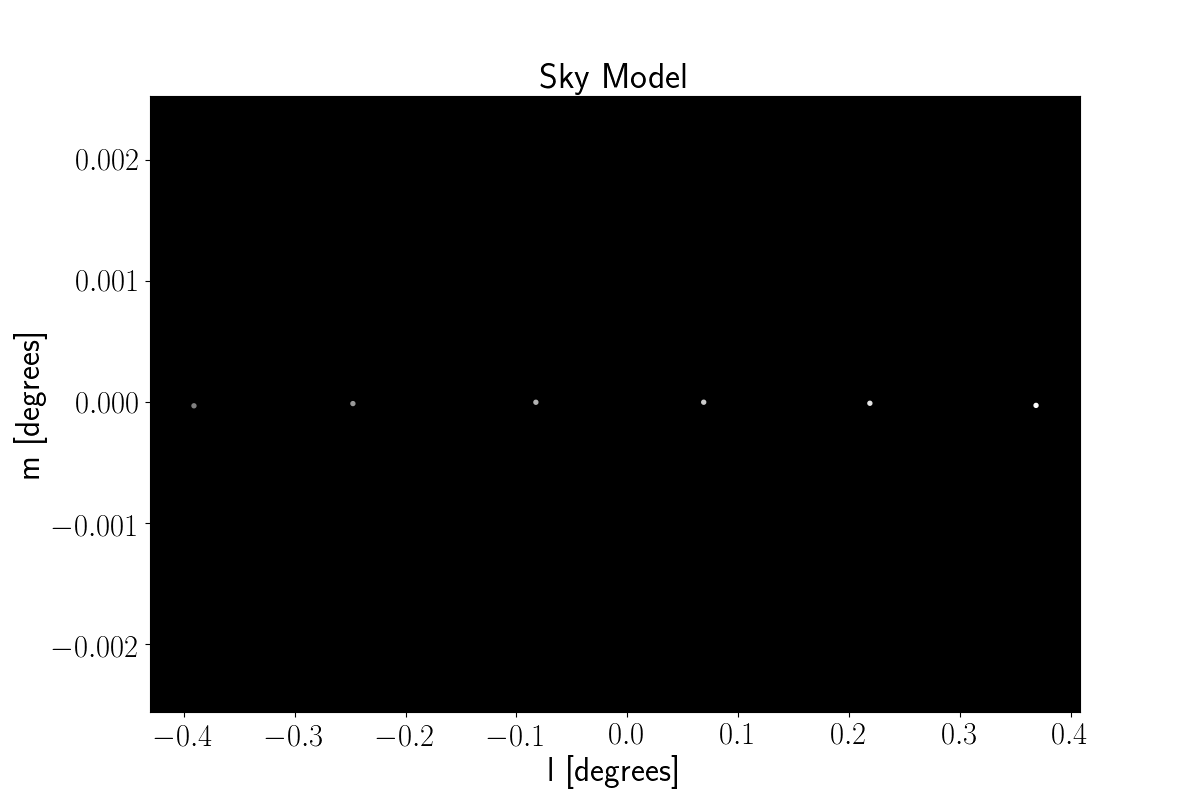
\includegraphics[width=\textwidth, scale=1]{images/TESTING_KAT7_LINEMODEL_SKY_MODEL.png}
    \vspace*{3mm}
    \caption{Testing input.}
    \label{fig:line_model}
  \end{subfigure}
  %
  \begin{subfigure}[b]{0.49\textwidth}
    \centering
    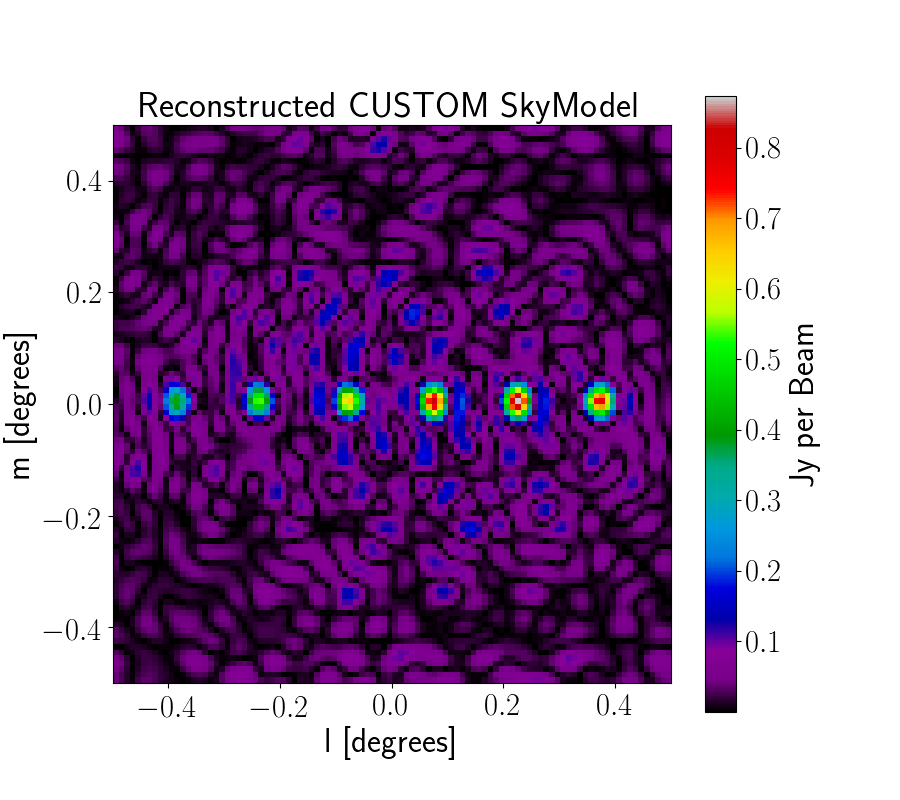
\includegraphics[scale=0.32]{images/TESTING_KAT7_LINEMODEL_RECON.png}
    \vspace*{-8mm}
    \caption{Testing output.}
    \label{fig:line_model_recon}
  \end{subfigure}
  \caption{Testing input and output.}
  \label{fig:Testing}
 \end{figure}

The user would then select a field of view of 1$^\circ$ and a cell size of 0.01$^\circ$.\\
The testing framework will generate an image based off the interferometer and sky model, the output of this testing will be figure \ref{fig:line_model_recon}.

This experiment can be applied to many interferometers, real or imaginary with any sky model, and provided the cell size and field of view are chosen correctly, the testing framework will produce an image that closely resembles the original sky model.\\
This shows that the pipeline is working correctly and that the images that are created by the TART section are correct.
